% Options for packages loaded elsewhere
\PassOptionsToPackage{unicode}{hyperref}
\PassOptionsToPackage{hyphens}{url}
\documentclass[
]{article}
\usepackage{xcolor}
\usepackage[margin=1in]{geometry}
\usepackage{amsmath,amssymb}
\setcounter{secnumdepth}{-\maxdimen} % remove section numbering
\usepackage{iftex}
\ifPDFTeX
  \usepackage[T1]{fontenc}
  \usepackage[utf8]{inputenc}
  \usepackage{textcomp} % provide euro and other symbols
\else % if luatex or xetex
  \usepackage{unicode-math} % this also loads fontspec
  \defaultfontfeatures{Scale=MatchLowercase}
  \defaultfontfeatures[\rmfamily]{Ligatures=TeX,Scale=1}
\fi
\usepackage{lmodern}
\ifPDFTeX\else
  % xetex/luatex font selection
\fi
% Use upquote if available, for straight quotes in verbatim environments
\IfFileExists{upquote.sty}{\usepackage{upquote}}{}
\IfFileExists{microtype.sty}{% use microtype if available
  \usepackage[]{microtype}
  \UseMicrotypeSet[protrusion]{basicmath} % disable protrusion for tt fonts
}{}
\makeatletter
\@ifundefined{KOMAClassName}{% if non-KOMA class
  \IfFileExists{parskip.sty}{%
    \usepackage{parskip}
  }{% else
    \setlength{\parindent}{0pt}
    \setlength{\parskip}{6pt plus 2pt minus 1pt}}
}{% if KOMA class
  \KOMAoptions{parskip=half}}
\makeatother
\usepackage{color}
\usepackage{fancyvrb}
\newcommand{\VerbBar}{|}
\newcommand{\VERB}{\Verb[commandchars=\\\{\}]}
\DefineVerbatimEnvironment{Highlighting}{Verbatim}{commandchars=\\\{\}}
% Add ',fontsize=\small' for more characters per line
\usepackage{framed}
\definecolor{shadecolor}{RGB}{248,248,248}
\newenvironment{Shaded}{\begin{snugshade}}{\end{snugshade}}
\newcommand{\AlertTok}[1]{\textcolor[rgb]{0.94,0.16,0.16}{#1}}
\newcommand{\AnnotationTok}[1]{\textcolor[rgb]{0.56,0.35,0.01}{\textbf{\textit{#1}}}}
\newcommand{\AttributeTok}[1]{\textcolor[rgb]{0.13,0.29,0.53}{#1}}
\newcommand{\BaseNTok}[1]{\textcolor[rgb]{0.00,0.00,0.81}{#1}}
\newcommand{\BuiltInTok}[1]{#1}
\newcommand{\CharTok}[1]{\textcolor[rgb]{0.31,0.60,0.02}{#1}}
\newcommand{\CommentTok}[1]{\textcolor[rgb]{0.56,0.35,0.01}{\textit{#1}}}
\newcommand{\CommentVarTok}[1]{\textcolor[rgb]{0.56,0.35,0.01}{\textbf{\textit{#1}}}}
\newcommand{\ConstantTok}[1]{\textcolor[rgb]{0.56,0.35,0.01}{#1}}
\newcommand{\ControlFlowTok}[1]{\textcolor[rgb]{0.13,0.29,0.53}{\textbf{#1}}}
\newcommand{\DataTypeTok}[1]{\textcolor[rgb]{0.13,0.29,0.53}{#1}}
\newcommand{\DecValTok}[1]{\textcolor[rgb]{0.00,0.00,0.81}{#1}}
\newcommand{\DocumentationTok}[1]{\textcolor[rgb]{0.56,0.35,0.01}{\textbf{\textit{#1}}}}
\newcommand{\ErrorTok}[1]{\textcolor[rgb]{0.64,0.00,0.00}{\textbf{#1}}}
\newcommand{\ExtensionTok}[1]{#1}
\newcommand{\FloatTok}[1]{\textcolor[rgb]{0.00,0.00,0.81}{#1}}
\newcommand{\FunctionTok}[1]{\textcolor[rgb]{0.13,0.29,0.53}{\textbf{#1}}}
\newcommand{\ImportTok}[1]{#1}
\newcommand{\InformationTok}[1]{\textcolor[rgb]{0.56,0.35,0.01}{\textbf{\textit{#1}}}}
\newcommand{\KeywordTok}[1]{\textcolor[rgb]{0.13,0.29,0.53}{\textbf{#1}}}
\newcommand{\NormalTok}[1]{#1}
\newcommand{\OperatorTok}[1]{\textcolor[rgb]{0.81,0.36,0.00}{\textbf{#1}}}
\newcommand{\OtherTok}[1]{\textcolor[rgb]{0.56,0.35,0.01}{#1}}
\newcommand{\PreprocessorTok}[1]{\textcolor[rgb]{0.56,0.35,0.01}{\textit{#1}}}
\newcommand{\RegionMarkerTok}[1]{#1}
\newcommand{\SpecialCharTok}[1]{\textcolor[rgb]{0.81,0.36,0.00}{\textbf{#1}}}
\newcommand{\SpecialStringTok}[1]{\textcolor[rgb]{0.31,0.60,0.02}{#1}}
\newcommand{\StringTok}[1]{\textcolor[rgb]{0.31,0.60,0.02}{#1}}
\newcommand{\VariableTok}[1]{\textcolor[rgb]{0.00,0.00,0.00}{#1}}
\newcommand{\VerbatimStringTok}[1]{\textcolor[rgb]{0.31,0.60,0.02}{#1}}
\newcommand{\WarningTok}[1]{\textcolor[rgb]{0.56,0.35,0.01}{\textbf{\textit{#1}}}}
\usepackage{graphicx}
\makeatletter
\newsavebox\pandoc@box
\newcommand*\pandocbounded[1]{% scales image to fit in text height/width
  \sbox\pandoc@box{#1}%
  \Gscale@div\@tempa{\textheight}{\dimexpr\ht\pandoc@box+\dp\pandoc@box\relax}%
  \Gscale@div\@tempb{\linewidth}{\wd\pandoc@box}%
  \ifdim\@tempb\p@<\@tempa\p@\let\@tempa\@tempb\fi% select the smaller of both
  \ifdim\@tempa\p@<\p@\scalebox{\@tempa}{\usebox\pandoc@box}%
  \else\usebox{\pandoc@box}%
  \fi%
}
% Set default figure placement to htbp
\def\fps@figure{htbp}
\makeatother
\setlength{\emergencystretch}{3em} % prevent overfull lines
\providecommand{\tightlist}{%
  \setlength{\itemsep}{0pt}\setlength{\parskip}{0pt}}
\usepackage{bookmark}
\IfFileExists{xurl.sty}{\usepackage{xurl}}{} % add URL line breaks if available
\urlstyle{same}
\hypersetup{
  pdftitle={MA213 - Fall 2025},
  hidelinks,
  pdfcreator={LaTeX via pandoc}}

\title{MA213 - Fall 2025}
\author{}
\date{\vspace{-2.5em}}

\begin{document}
\maketitle

\section{Basic Statistics and
Probability}\label{basic-statistics-and-probability}

\subsection{\texorpdfstring{\textbf{Lab Session 4: Simulation and
probability}}{Lab Session 4: Simulation and probability}}\label{lab-session-4-simulation-and-probability}

In this lab session, we will go over central limit theorem. Can we
verify central limit theorem by simulation?

\subsection{Pre-lab activities}\label{pre-lab-activities}

\begin{itemize}
\item
  The role of sampling distribution : Why do we care about sampling
  distribution?

  \begin{enumerate}
  \def\labelenumi{\arabic{enumi}.}
  \tightlist
  \item
    What is sampling distribution?
  \end{enumerate}

  -\textgreater{} In inferential statistics, we estimate the
  characteristics of the population parameter by using characteristics
  of sample (statistic).

  -\textgreater{} The distribution of the statistic obtained from sample
  is called sampling distribution.
\end{itemize}

\pandocbounded{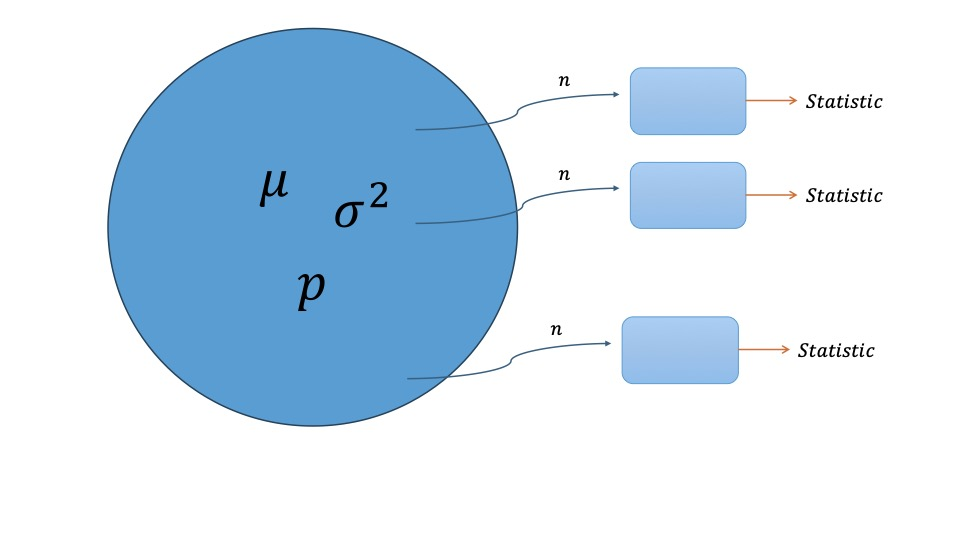
\includegraphics[keepaspectratio]{Sampling_diag.jpg}}

\subsection{Lab activities}\label{lab-activities}

We have a hypothetical population that are

\begin{Shaded}
\begin{Highlighting}[]
\NormalTok{pop }\OtherTok{\textless{}{-}} \FunctionTok{c}\NormalTok{(}\FunctionTok{rep}\NormalTok{(}\StringTok{"Apple"}\NormalTok{, }\DecValTok{10}\NormalTok{), }\FunctionTok{rep}\NormalTok{(}\StringTok{"Android"}\NormalTok{, }\DecValTok{4}\NormalTok{))}
\end{Highlighting}
\end{Shaded}

So that the true proportion of having apple device is
\(p=\frac{10}{14}\).

Let's sample them with \(n=5\). What is the sampling distribution look
like?

\begin{enumerate}
\def\labelenumi{\arabic{enumi}.}
\item
  Let's sample them and assign it to an object \texttt{p\_hat} .

  (hint : use \texttt{sample()} and how many are there are apple ?)
\item
  What is the sampling distribution look like? (obtain a vector
  \texttt{p\_hat})

  (hint : Use \texttt{for\ loop} )
\item
  Using \texttt{p\_hat} vector, show sampling distribution of the
  statistic.
\item
  Now you are given much bigger hypothetical population where

\begin{Shaded}
\begin{Highlighting}[]
\NormalTok{pop }\OtherTok{\textless{}{-}} \FunctionTok{c}\NormalTok{(}\FunctionTok{rep}\NormalTok{(}\StringTok{"Apple"}\NormalTok{, }\DecValTok{1000}\NormalTok{), }\FunctionTok{rep}\NormalTok{(}\StringTok{"Android"}\NormalTok{, }\DecValTok{400}\NormalTok{))}
\end{Highlighting}
\end{Shaded}

  Now you know that the true population proportion is \(p=0.7142\) .

  Let's make a function \texttt{my\_sample} to give shape of
  distribution. (input \texttt{n}, output vector \texttt{p\_hat}).
\item
  Using \texttt{my\_sample} function, show the sampling distribution of
  the statistic. Change \texttt{n} from 10 to 100. What do you conclude?
\end{enumerate}

\subsubsection{Post-lab activities}\label{post-lab-activities}

Recent statistics suggest that 10\% of Americans rely on Social Network
Sites (SNSs). We are going to have a simulation study if we can verify
that CLT really works in this case too. Let's assume that US population
is 300,000 for calculation purposes.

Please name your submission as \texttt{lab4.R}

\begin{enumerate}
\def\labelenumi{\arabic{enumi}.}
\setcounter{enumi}{-1}
\item
  execute this \texttt{set.seed(213)}
\item
  Produce population data and assign it \texttt{population} object.
\item
  Obtain mean and standard deviation of the population and assign them
  to \texttt{mean\_pop} and \texttt{sd\_pop} accordingly.
\item
  Get the sample mean data for \(n=10\) with \(k=100\) iterations.
  Assign the mean and standard deviation of the sample mean data to
  \texttt{mean\_sample} and \texttt{sd\_sample}.
\item
  Do one more time with the sample mean data for \(n=50\) with \(k=100\)
  iterations. Assign the mean and standard deviation of the sample mean
  data to \texttt{mean\_sample2} and \texttt{sd\_sample2}.
\item
  (Extra)

  5.1) Show the shape of the sample proportion with n=10, k=1000.

  5.2) Show the shape of the sample proportion with n=1000, k=1000.
\end{enumerate}

\end{document}
